\chapter{Projekt rozwiązania}
\label{chap:hl-arch}

        Niniejszy rozdział opisuje koncept rozwiązania, który powstał w ramach pracy. Ogólny zarys konceptu działania systemu przedstawiony jest na rysnku \ref{fig:door}.

        \begin{figure}[]
                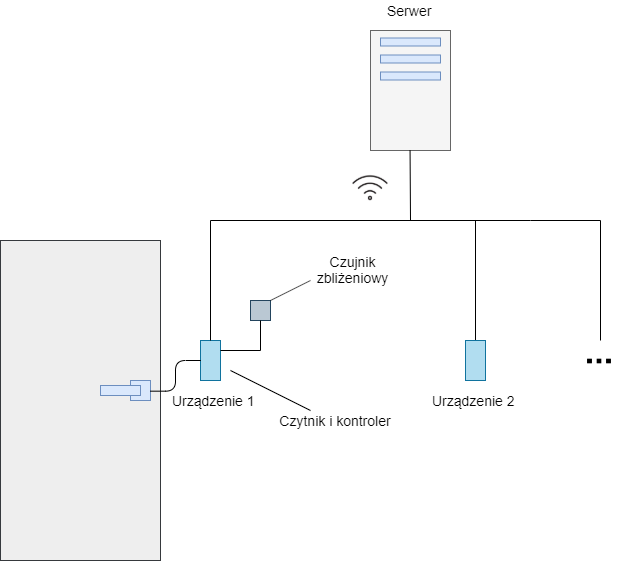
\includegraphics[width=\linewidth]{chapters/images/door2.png}
                \caption{Koncept systemu kontroli dostępu}
                \label{fig:door}
        \end{figure}

        \section{Architektura systemu}
                W ramach systemu można wyodrębnić następujące podsystemy:
                \begin{enumerate}
                        \item Podsystem sterowania zamkiem,
                        \item Podsystem autoryzacji,
                        \item Podsystem zarządzania.
                \end{enumerate}

                Podsystemy te istnieją w ramach komponentów sprzętowych. Są to:
                \begin{enumerate}
                        \item Komponent sterujący zamkiem (inaczej: kontroler, układ zamka),
                        \item Komponent serwera.
                \end{enumerate}

                Komponenty te zostały krótko omówione w kolejnych punktach. Ogólna sprzętowa architektura systemu z podziałem na komponenty sprzętowe oraz przynależne im podsystemy przedstawiona została na rysunku \ref{fig:hl-arch}.

                \begin{figure}[]
                        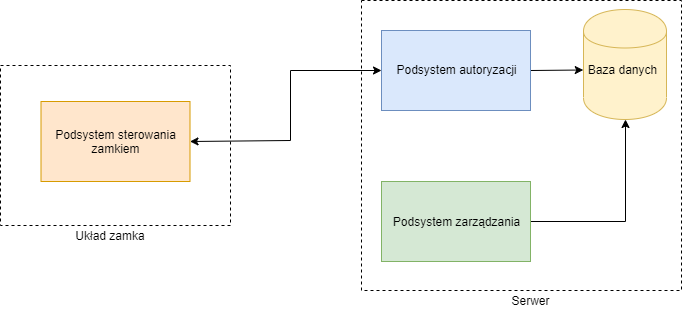
\includegraphics[width=\linewidth]{chapters/images/hl-arch3.png}
                        \caption{Architektura systemu}
                        \label{fig:hl-arch}
                \end{figure}

                \subsection{Komponent sterujący zamkiem}
                        Komponent sterujący zamkiem składa się z mikrokontrolera, czujnika ruchu oraz czytnika RFID. Mikrokontroler odpowiada za sterowanie peryferiami, zarządza ich zasilaniem, inicjuje i przeprowadza bezprzewodową komunikację z serwerem i steruje samym zamkiem na podstawie otrzymanych od serwera danych. Podsystem sterowania zamkiem zlokalizowany jest w całości w tym komponencie (patrz rysunek \ref{fig:hl-arch}). Architektura układu zamka została przedstawiona na rysunku \ref{fig:lock-arch}. 

                        \begin{figure}
                                \centering
                                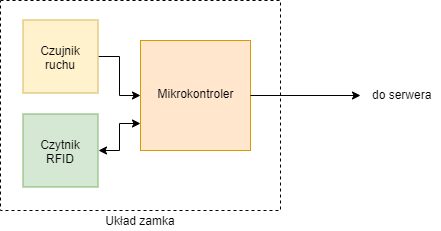
\includegraphics[width=0.7\textwidth]{chapters/images/lock.png}
                                \caption{Architektura układu zamka}
                                \label{fig:lock-arch}
                        \end{figure}

                \subsection{Serwer główny}
                        W ramach komponentu serwera działają dwa podsystemy funkcjonalne: podsystem autoryzacji, odpowiedzialny za podjęcie decyzji o przyznaniu lub odmowie dostępu na podstawie danych odebranych od podsystemu sterowania zamkiem, oraz podsystem zarządzania, odpowiedzialny za zbieranie oraz prezentację danych użytkownikowi.

                \subsubsection{Baza danych}
                        Częścią komponentu serwera jest baza danych. Nie jest jednak konieczne, aby pozostawała ona fizycznie na tej samej maszynie. W przypadku całkowitego rozdzielenia serwera danych od serwera autoryzacji skalowalność systemu znacząco wzrośnie.

                \subsubsection{Podsystem autoryzacji}
                        Zadaniem podsystemu autoryzacji jest podjęcie decyzji o przyznaniu bądź odmowie dostępu na podstawie otrzymanych danych. Podsystem komunikuje się z bazą danych w celu uzyskania informacji na temat autoryzowanych kart.

                \subsubsection{Podsystem zarządzania}
                        Zadaniem podsystemu zarządzania jest umożliwienie użytkownikowi systemu wglądu do danych takich jak historia prób dostępu, zbiór zamków, kart oraz powiązań między nimi, oraz stan poszczególnych zamków.

        \section{Zasada działania}
                Kontroler wbudowany w zamek pozostaje uśpiony do momentu wykrycia ruchu w pobliżu przez wbudowany czujnik ruchu. Po wybudzeniu nawiązuje bezpieczne połączenie z serwerem autoryzacji, jednocześnie zasilając czytnik RFID oraz oczekując na zbliżenie do niego karty. Gdy karta zostanie zbliżona, kontroler przesyła odczytany z niej numer identyfikacyjny do serwera, korzystając z nawiązanego wcześniej połączenia. Serwer podejmuje decyzję, którą jest przyznanie bądź odmowa dostępu, porównując odebrany numer identyfikacyjny z zawartością bazy danych, a następnie przesyła informację zwrotną do kontrolera. Jeżeli podjęto decyzję o przyznaniu dostępu, kontroler wysyła sygnał otwarcia zamka oraz sygnalizuje powodzenie. Jeżeli podjęto decyzję o odmowie dostępu, kontroler sygnalizuje niepowodzenie. Diagram sekwencji przedstawiony jest na rysunku \ref{fig:sequence1}.

                \begin{figure}[]
                        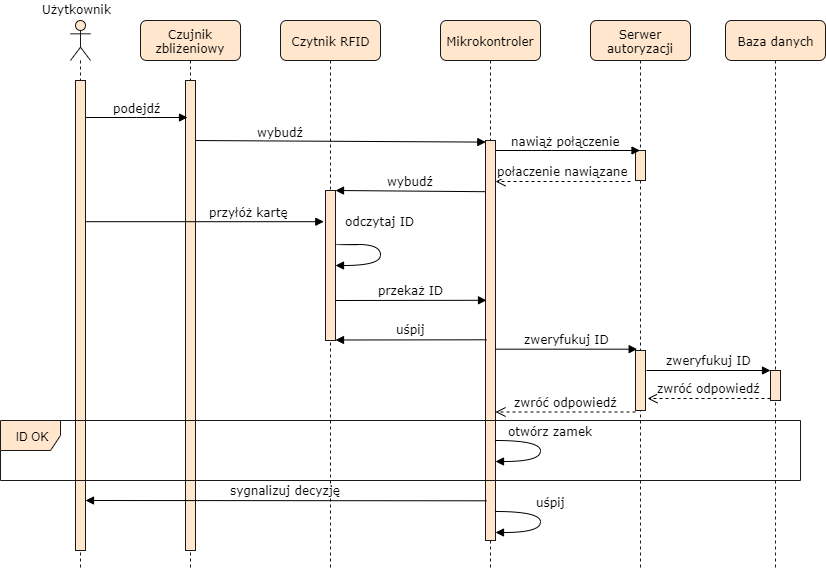
\includegraphics[width=\linewidth]{chapters/images/sequence1.png}
                        \caption{Diagram sekwencji ukazujący zasadę działania systemu}
                        \label{fig:sequence1}
                \end{figure}

